%%%%%%%%%%%%%%%%%%%%%%%%%%%%%%%%%%%%%%%%%%%%%%%%%%%%%%%%
%%%%%%%%%%%%%%%%%%%%%%%%%%%%%%%%%%%%%%%%%%%%%%%%%%%%%%%%
%%%%%%%%%%%%%%%%%%%%%%%%%%%%%%%%%%%%%%%%%%%%%%%%%%%%%%%%
\chapter{Statistics}
\label{chap:stats}

%%%%%%%%%%%%%%%%%%%%%%%%%%%%%%%%%%%%%%%%%%%%%%%%%%%%%%%%
%%%%%%%%%%%%%%%%%%%%%%%%%%%%%%%%%%%%%%%%%%%%%%%%%%%%%%%%
\section{Bayes' Theorem}
\label{stats:Bayes}

Bayes' theorem follows from the probability of the intersection of two events $A$ and $B$:

\begin{equation}\label{eq:stats:intersection}
P\left(A \cap B\right) = P\left(A \mid B\right) P\left(B\right) = P\left(B \mid A\right) P\left(A\right).
\end{equation}

\noindent Dividing by $P\left(B\right)$ we have:

\begin{equation}\label{eq:stats:Bayes}
\begin{split}
P\left(A \mid B\right) &= \frac{P\left(B \mid A\right) P\left(A\right)}{P\left(B\right)}\,, \\
&= \frac{P\left(B \mid A_{i}\right) P\left(A_{i}\right)}{\sum_{j} P\left(B \mid A_{j}\right)P\left(A_{j}\right)}\,, \\
\text{Posterior} &= \frac{\text{Likelihood} \times \text{Prior}}{\text{Normalization}}\,.
\end{split}
\end{equation}

%%%%%%%%%%%%%%%%%%%%%%%%%%%%%%%%%%%%%%%%%%%%%%%%%%%%%%%%
\subsubsection{Example: Medical Testing}
\label{stats:Bayes:medical_test}

Example: Testing for disease with a \SI{2}{\percent} incidence rate in the wider population.
The test has a \SI{99}{\percent} true positive rate and a \SI{5}{\percent} false positive rate.
What is the probability an individual has the disease if their test is positive?

% https://www.wolframalpha.com/input/?i=(0.99*0.02)%2F((0.99*0.02)%2B(0.05*(1%E2%88%920.02)))
\begin{equation}\label{eq:stats:Bayes:medical_test_1}
\begin{split}
P\left(\text{Infected} \mid +\right) &= \frac{P\left(+ \mid \text{Infected}\right) P\left(\text{Infected}\right)}{P\left(+\right)}\,, \\
 &= \frac{P\left(+ \mid \text{Infected}\right) P\left(\text{Infected}\right)}{
P\left(+ \mid \text{Infected}\right)P\left(\text{Infected}\right) + P\left(+ \mid \text{Healthy}\right)P\left(\text{Healthy}\right)}\,, \\
&= \frac{\num{0.99} \times \num{0.02}}{\num{0.99} \times \num{0.02} + \num{0.05} \times \left(1-\num{0.02}\right)}\,, \\
&\approx \num{0.288}\,.
\end{split}
\end{equation}

\noindent And if we then run a second, independent, test which also comes back positive?

% https://www.wolframalpha.com/input/?i=(0.99*0.288)%2F((0.99*0.288)%2B(0.05*(1%E2%88%920.288)))
\begin{equation}\label{eq:stats:Bayes:medical_test_2}
\begin{split}
P\left(\text{Infected} \mid ++\right) &= \frac{P\left(+ \mid \text{Infected}\right) P\left(\text{Infected} \mid +\right)}{
P\left(+ \mid \text{Infected}\right)P\left(\text{Infected} \mid +\right) + P\left(+ \mid \text{Healthy}\right)P\left(\text{Healthy} \mid +\right)}\,, \\
&= \frac{\num{0.99} \times \num{0.288}}{\num{0.99} \times \num{0.288} + \num{0.05} \times \left(1-\num{0.288}\right)}\,, \\
&\approx \num{0.889}\,.
\end{split}
\end{equation}

\noindent Note that if we ran both tests the first time we would still have:

% https://www.wolframalpha.com/input/?i=(0.99%5E2*0.02)%2F((0.99%5E2*0.02)%2B(0.05%5E2*(1%E2%88%920.02)))
\begin{equation}\label{eq:stats:Bayes:medical_test_3}
\begin{split}
P\left(\text{Infected} \mid ++\right) &= \frac{P\left(++ \mid \text{Infected}\right) P\left(\text{Infected}\right)}{P\left(++\right)}\,, \\
&= \frac{\num{0.99}^{2} \times \num{0.02}}{\num{0.99}^{2} \times \num{0.02} + \num{0.05}^{2} \times \left(1-\num{0.02}\right)}\,, \\
&\approx \num{0.889}\,.
\end{split}
\end{equation}

%%%%%%%%%%%%%%%%%%%%%%%%%%%%%%%%%%%%%%%%%%%%%%%%%%%%%%%%
\subsubsection{Example: Biased Coin}
\label{stats:Bayes:biased_coin}

Consider the case of a bag of $n$ fair coins and $m$ biased coins.
Let $P\left(H \mid \stcomp{F}\right) \equiv p_{H}$ be the \apriori probability of heads $H$ for an biased coin $\stcomp{F}$.
Drawing one coin from the bag, you flip it multiple times recording $h$ heads and $t$ tails.
What is the probability you have drawn an biased coin, $P\left(\stcomp{F} \mid h,t\right)$?

\begin{equation}\label{eq:stats:Bayes:biased_coin_setup}
\begin{gathered}
P\left(F\right) = \frac{n}{n+m}\,,\quad P\left(\stcomp{F}\right) = \frac{m}{n+m}\,, \\
P\left(H \mid F\right) = \frac{1}{2}\,,\quad P\left(h,t \mid F\right) = \left(\frac{1}{2}\right)^{h}\,\left(\frac{1}{2}\right)^{t} = \frac{1}{2^{h+t}}\,, \\
P\left(h,t \mid \stcomp{F}\right) = P\left(H \mid \stcomp{F}\right)^{h} P\left(\stcomp{H} \mid \stcomp{F}\right)^{t} = p_{H}^{h} \left(1-p_{H}\right)^{t}.
\end{gathered}
\end{equation}

\begin{equation}\label{eq:stats:Bayes:biased_coin_solution}
\begin{split}
P\left(\stcomp{F} \mid h,t\right) &= \frac{
P\left(h,t \mid \stcomp{F}\right) P\left(\stcomp{F}\right)}{
P\left(h,t \mid \stcomp{F}\right) P\left(\stcomp{F}\right) + P\left(h,t \mid F\right) P\left(F\right)} \\
&= \frac{
m\,p_{H}^{h} \left(1-p_{H}\right)^{t}}{
m\,p_{H}^{h} \left(1-p_{H}\right)^{t} + n\,2^{-h-t}}\,.
\end{split}
\end{equation}

Some example values are provided in \cref{tab:Bayes:biased_coin}.

\begin{table}[H]
\centering
\begingroup
\renewcommand*{\arraystretch}{1}
% $m = 50$, $n = 50$

\begin{tabular}{c c c c}
\hline
$h$ & $t$ & $p_{H}$ & $P\left(\stcomp{F} \mid h,t\right)$ \\
\hline
\hline
10 & 0 & 1.00 & 0.99902 \\
10 & 0 & 0.80 & 0.99099 \\
10 & 0 & 0.60 & 0.86095 \\
\hline
7 & 3 & 0.99 & 0.00095 \\
7 & 3 & 0.80 & 0.63208 \\
7 & 3 & 0.60 & 0.64722 \\
\hline
5 & 5 & 0.99 & 0.00000 \\
5 & 5 & 0.80 & 0.09696 \\
5 & 5 & 0.60 & 0.44915 \\
\hline
75 & 25 & 0.99 & 0.00000 \\
75 & 25 & 0.80 & 1.00000 \\
75 & 25 & 0.60 & 0.99970 \\
\hline
\end{tabular}
\endgroup
\caption{
$P\left(\stcomp{F} \mid h,t\right)$ for various values of $h$, $t$, and $p_{H}$ when $m = 50$, $n = 50$.
}
\label{tab:Bayes:biased_coin}
\end{table}

%%%%%%%%%%%%%%%%%%%%%%%%%%%%%%%%%%%%%%%%%%%%%%%%%%%%%%%%
%%%%%%%%%%%%%%%%%%%%%%%%%%%%%%%%%%%%%%%%%%%%%%%%%%%%%%%%
\section{Coin Problems}
\label{stats:coin_problems}

%%%%%%%%%%%%%%%%%%%%%%%%%%%%%%%%%%%%%%%%%%%%%%%%%%%%%%%%
\subsection{Making an Biased Coin Fair}
\label{stats:coin_problems:biased_to_fair}
% https://fivethirtyeight.com/features/can-you-make-an-unfair-coin-fair/
% https://fivethirtyeight.com/features/can-you-snatch-defeat-from-the-jaws-of-victory/
% https://youtu.be/-SANBbv0-Hw
% https://math.stackexchange.com/a/146614 for additional references

If we are given an biased coin with $P\left(H\right) = p \neq \num{0.5}$
we can construct a fair coin\footnote{The solution is credited to John von Neumann, who really did work on everything!} by
flipping the biased coin $m$ times and selecting outcomes with an equal probability of occurring, while disregarding all other outcomes.
For example, with $m=2$ flips we have the outcomes listed in \cref{tab:coin_problems:biased_to_fair:m2_outcomes}:

\begin{table}[H]
\centering
\begingroup
\renewcommand*{\arraystretch}{1}
\begin{tabular}{c c c c}
\hline
Outcome & $P\left(\text{Outcome}\right)$ & Assignment \\
\hline
\hline
$HH$ & $p^{2}$ & Disregard \\
$HT$ & $p\left(1-p\right)$ & H \\
$TH$ & $\left(1-p\right)p$ & T \\
$TT$ & $\left(1-p\right)^{2}$ & Disregard \\
\end{tabular}

\endgroup
\caption{
Making an biased coin fair in $m=2$ flips.
}
\label{tab:coin_problems:biased_to_fair:m2_outcomes}
\end{table}

Note that we are disregarding $p^{2} + \left(1-p\right)^{2}$ percent of flips
and this method will become increasingly inefficient as $p$ moves away from $\num{0.5}$.
We can improve the efficiency by increasing $m$ and reassigning the
outcomes\footnote{For $m = \num{4}$, disregard $P\left(HHHH \parallel TTTT\right) = p^{4} + \left(1-p\right)^{4} < p^{2} + \left(1-p\right)^{2}$,\newline
$HT \parallel HHHT \parallel HHTT \parallel TTHT \to H$,\newline
$TH \parallel TTTH \parallel TTHH \parallel HHTH \to T = H^{-1}$.} such that
we decrease the average number of flips required.
If we need to simulate something with more outcomes, like a 6 sided die,
we can increase $m$ until we have enough equal outcomes, or combinations of outcomes.

We can also ask, for what values of $p$ is a fair outcome ensured in $m$ flips?
To solve, create $P\left(\text{Outcome}\right)$ for all possible outcomes of $m$ flips.
Then, sum all possible combinations\footnote{Excluding the combination with all outcomes where $\sum P\left(\text{Outcome}\right) = 1$.} of $P\left(\text{Outcome}\right)$
and try to solve $\sum P\left(\text{Outcome}\right) = \num{0.5}$.
This partitions the outcomes into two assignments without disregarding any outcomes, \ie no flips are wasted.
For example, with $m=2$ and \cref{tab:coin_problems:biased_to_fair:m2_outcomes}, we solve
$p^{2}$, $p\left(1-p\right)$, $\left(1-p\right)^{2}$,
$p^{2} + p\left(1-p\right)$, $p\left(1-p\right) + \left(1-p\right)^{2}$, and $p^{2} + \left(1-p\right)^{2} = \num{0.5}$
separately for $0<p<1$.
The valid $p$ are then
$p = 1/\sqrt{2}$ with $HH \to H$,
$p = \num{0.5}$ with $HH \parallel TT \to H$,
and $p = 1 - 1/\sqrt{2}$ with $TT \to H$;
everything else $\to T$.

%%%%%%%%%%%%%%%%%%%%%%%%%%%%%%%%%%%%%%%%%%%%%%%%%%%%%%%%
\subsection{Making an Fair Coin Biased}
\label{stats:coin_problems:fair_to_biased}

In the opposite direction, we can also make a fair coin biased
with $P\left(H\right) = p = 1/N$ by flipping it
$m = \text{ceil}\left(\log_{2}N\right)$ times
and reassigning the outcomes such that $H^{m} \to H$,
$N-1$ other outcomes $\to T$, and we disregard any remaining $m-N$ outcomes.

%%%%%%%%%%%%%%%%%%%%%%%%%%%%%%%%%%%%%%%%%%%%%%%%%%%%%%%%
%%%%%%%%%%%%%%%%%%%%%%%%%%%%%%%%%%%%%%%%%%%%%%%%%%%%%%%%
\section{Uniform Distribution}
\label{stats:uniform}

The uniform distribution, \cref{eq:stats:uniform:P} and \cref{fig:dist:uniform},
is the simplest probability distribution
having a constant probability $1/(a+b)$ over the interval $a$ to $b$.

\begin{equation}\label{eq:stats:uniform:P}
P\left(x;\,a,\,b\right) = \begin{cases}
\frac{1}{b-a} & a \leq x \leq b \,, \\
0 & \text{otherwise} \,,
\end{cases}
\end{equation}

It is illustrative to compute the mean and variance of the uniform distribution from $P(x)$ directly:

\begin{subequations}\label{eq:stats:uniform:mean_variance}
\begin{align}
\expval{x} &= \int_{-\infty}^{\infty} x P\left(x\right) \, \dd{x} = \frac{1}{b-a} \int_{a}^{b} x \, \dd{x} = \frac{1}{2(b-a)}\left(b^{2} - a^{2}\right) = \frac{1}{2}\left(a + b\right)\,, \label{eq:stats:uniform:mean_variance:mean} \\
\variance{x} &= \expval{x^{2}} - \expval{x}^{2} = \frac{1}{b-a} \int_{a}^{b} x^{2} \, \dd{x} - \expval{x}^{2} = \cdots = \frac{1}{12}\left(b-a\right)^{2}\,. \label{eq:stats:uniform:mean_variance:variance}
\end{align}
\end{subequations}

%%%%%%%%%%%%%%%%%%%%%%%%%%%%%%%%%%%%%%%%%%%%%%%%%%%%%%%%
%%%%%%%%%%%%%%%%%%%%%%%%%%%%%%%%%%%%%%%%%%%%%%%%%%%%%%%%
\section{Binomial Distribution}
\label{stats:binomial}

The binomial distribution, \cref{eq:stats:binomial:P} and \cref{fig:dist:binomial},
gives the probability of observing $k$ successes in $n$ independent Boolean trials,
when $p$ is the probability of success in any one trial.

\begin{subequations}\label{eq:stats:binomial}
\begin{align}
P\left(k;\,n,p\right) &= {n \choose k}p^{k} \left(1-p\right)^{n-k}, \label{eq:stats:binomial:P} \\
{n \choose k} &\equiv \frac{n!}{k!\left(n-k\right)!}\,. \label{eq:stats:binomial_coefficient}
\end{align}
\end{subequations}

\noindent Here \cref{eq:stats:binomial_coefficient} is the binomial coefficient,
representing the number of unordered combinations\footnote{There are
$P_{k}^{n} = n! / \left(n-k\right)$ ways of selecting an ordered subset,
or permutation, of $k$ from $n$.} which select $k$ elements from $n$ elements; $n$ choose $k$.

The mean and variance of the binomial distribution are:

\begin{subequations}\label{eq:stats:binomial:mean_variance}
\begin{align}
\expval{k} &= \sum_{k=0}^{n} k P\left(k;\,n,p\right) = n p\,, \label{eq:stats:binomial:mean} \\
\sigma^{2} &= n p\left(1-p\right). \label{eq:stats:binomial:variance}
\end{align}
\end{subequations}

\subsubsection{Bernoulli Distribution}
\label{stats:binomial:bernoulli}

For the special case when $n=1$, we have the Bernoulli distribution:

\begin{equation}\label{eq:stats:bernoulli}
P\left(k;\,p\right) = p^{k} \left(1-p\right)^{1-k}, \quad \expval{k} = p\,, \quad \sigma^{2} = p\left(1-p\right).
\end{equation}

\subsubsection{Negative Binomial Distribution}
\label{stats:binomial:negative}

If we are interested in the probability of
observing $k$ successes before we observe $r$ failures,
we can slightly modify the binomial distribution to be
the ``negative''\footnote{Negative as in ${k+r-1 \choose k} = \left(-1\right)^{k} {-r \choose k}$.} binomial distribution:

\begin{subequations}\label{eq:stats:binomial:neg:P}
\begin{align}
P\left(k;\,r,p\right) = {k+r-1 \choose k} p^{k} \left(1-p\right)^{r}\,,
\end{align}
\end{subequations}

\noindent where $p$ is still the probability of a success.
Note that since we stop on the $r^{\text{th}}$ failure,
we need to only arrange the $k$ successes in the first $k+r-1$ trials.

The mean and variance are then:

\begin{subequations}\label{eq:stats:binomial:neg:mean_variance}
\begin{align}
\expval{k} &= r p / \left(1-p\right)\,, \label{eq:stats:binomial:neg:mean} \\
\sigma^{2} &= r p / \left(1-p\right)^{2}. \label{eq:stats:binomial:neg:variance}
\end{align}
\end{subequations}

%%%%%%%%%%%%%%%%%%%%%%%%%%%%%%%%%%%%%%%%%%%%%%%%%%%%%%%%
%%%%%%%%%%%%%%%%%%%%%%%%%%%%%%%%%%%%%%%%%%%%%%%%%%%%%%%%
\section{Poisson Distribution}
\label{stats:poisson}

For rare processes with $p \ll 1$, and thus $\lambda \equiv n\,p \ll 1$,
the binomial distribution reduces\footnote{See
one \href{https://medium.com/@andrew.chamberlain/deriving-the-poisson-distribution-from-the-binomial-distribution-840cc1668239}{derivation here}.} to the
Poisson distribution:

\begin{equation}\label{eq:stats:poisson:P}
P\left(k;\,\lambda\right) = \frac{\lambda^{k}}{k!}\,e^{-\lambda}\,. \\
\end{equation}

\noindent Note that here $\lambda$ is continuous, while $k$ is still an integer.
A plot of the distribution can be found in \cref{fig:dist:poisson}.

Interestingly, the mean and variance of the Poisson distribution are identical and equal to $\lambda$:

\begin{equation}\label{eq:stats:poisson:mean_variance}
\expval{k} = \sigma^{2} = \lambda\,.
\end{equation}

\subsubsection{Example: Cars Driving By}
\label{stats:poisson:cars}
% TODO add

%%%%%%%%%%%%%%%%%%%%%%%%%%%%%%%%%%%%%%%%%%%%%%%%%%%%%%%%
%%%%%%%%%%%%%%%%%%%%%%%%%%%%%%%%%%%%%%%%%%%%%%%%%%%%%%%%
\section{Exponential Distribution}
\label{stats:exp}

If we sample the time intervals between Poisson distributed events
we arrive at the exponential distribution,

\begin{equation}\label{eq:stats:exp:P}
P\left(x;\,\lambda\right) = \begin{cases}
\lambda e^{-\lambda x} & x \geq 0 \,, \\
0 & x < 0 \,,
\end{cases}
\end{equation}

\noindent with rate parameter $\lambda$.
A plot of the distribution can be found in \cref{fig:dist:exp}.

The mean and standard deviation of the exponential distribution are identical and equal to $1/\lambda$:

\begin{equation}\label{eq:stats:exp:mean_variance}
\expval{x} = \sigma = \frac{1}{\lambda}\,, \quad \sigma^{2} = \frac{1}{\lambda^{2}}\,.
\end{equation}

The exponential distribution is memoryless\footnote{The exponential (geometric) distribution is the only real number (integer) memoryless probability distribution.} \cref{eq:stats:exp:memoryless},
\ie the time until a future event occurs does not depend on the time elapsed at the present.

\begin{equation}\label{eq:stats:exp:memoryless}
P\left(T > t + s \mid T > s\right) = P\left(T > t\right)\,, \quad \forall s,t \geq 0.
\end{equation}

%%%%%%%%%%%%%%%%%%%%%%%%%%%%%%%%%%%%%%%%%%%%%%%%%%%%%%%%
%%%%%%%%%%%%%%%%%%%%%%%%%%%%%%%%%%%%%%%%%%%%%%%%%%%%%%%%
\section{Gaussian Distribution}
\label{stats:gaus}

In the other direction, for common processes $\mu \equiv n\,p \gg 1$,
the binomial distribution becomes\footnote{See
one \href{http://scipp.ucsc.edu/~haber/ph116C/NormalApprox.pdf}{derivation here}.} the
well-known Gaussian, or normal, distribution,

\begin{equation}\label{eq:stats:gaus:P}
P\left(x;\,\mu,\sigma\right) = \frac{1}{\sqrt{2\pi}\,\sigma} \exp\left( -\frac{1}{2} \left(\frac{x-\mu}{\sigma}\right)^{2} \right)\,,
\end{equation}

\noindent with mean $\mu$ and variance $\sigma^{2}$.
A plot of the distribution can be found in \cref{fig:dist:gaus}.

It is helpful to remember that

\begin{equation}\label{eq:stats:gaus:sigmas}
\begin{split}
\mu \pm 1\sigma &\approx \SI{68}{\percent}\,, \\
\mu \pm 2\sigma &\approx \SI{95}{\percent}\,, \\
\mu \pm 3\sigma &\approx \SI{99}{\percent}\,,
\end{split}
\end{equation}

\noindent while the full width at half maximum (FWHM) $\Gamma = 2\sqrt{2 \ln{2}}\,\sigma \approx \num{2.355} \sigma$.
Note that the standard normal distribution has $\mu = 0$ and $\sigma =1$.

%%%%%%%%%%%%%%%%%%%%%%%%%%%%%%%%%%%%%%%%%%%%%%%%%%%%%%%%
%%%%%%%%%%%%%%%%%%%%%%%%%%%%%%%%%%%%%%%%%%%%%%%%%%%%%%%%
\section{Student's \texorpdfstring{$t$}{t}-Distribution}
\label{stats:t_dist}

If we take a sample of size $m$ from a normal distribution
we arrive at Student's $t$-distribution.
Letting $\nu = m-1$ be the number of degrees of freedom,
Student's $t$-distribution has the form:

\begin{equation}\label{eq:stats:t_dist:P}
P\left(t;\,\nu\right) = \frac{
\Gamma\left(\frac{\nu+1}{2}\right)
}{
\sqrt{\nu \pi}\,\Gamma\left(\frac{\nu}{2}\right)
} \left(1+\frac{t^{2}}{\nu}\right)^{-\frac{\nu+1}{2}}\,,
\end{equation}

\noindent where $\Gamma\left(z\right)$ is the gamma function\footnote{$\Gamma\left(z\right) = \int_{0}^{\infty} x^{z-1} e^{-x} \, \dd{x}$,
which simplifies to $\Gamma\left(n\right)=\left(n-1\right)!$ for integer $n$.}.
The distribution, \cref{fig:dist:student_t}, has a mean of \num{0} for $\nu > 1$,
and variance of $\infty$ for $\nu =2$ and $\nu / \left(\nu-2\right)$ for $\nu > 2$.

%%%%%%%%%%%%%%%%%%%%%%%%%%%%%%%%%%%%%%%%%%%%%%%%%%%%%%%%
%%%%%%%%%%%%%%%%%%%%%%%%%%%%%%%%%%%%%%%%%%%%%%%%%%%%%%%%
\section{\texorpdfstring{$\chi^{2}$-Distribution}{Chi-Squared Distribution}}
\label{stats:chi2_dist}

The $\chi^{2}$-distribution with $\nu$ degrees of freedom,
\cref{eq:stats:chi2_dist:P} and \cref{fig:dist:chi2},
is created by summing the squares of $\nu$ independent standard normal random variables.
It therefore has a mean of $\nu$ and variance of $2\nu$, and is
primary useful for conducting $\chi^{2}$-tests.

\begin{equation}\label{eq:stats:chi2_dist:P}
P\left(x;\,\nu\right) = \frac{
x^{\frac{\nu}{2} - 1} e^{-\frac{x}{2}}
}{
2^{\frac{\nu}{2}} \Gamma\left(\frac{\nu}{2}\right)}.
\end{equation}

%%%%%%%%%%%%%%%%%%%%%%%%%%%%%%%%%%%%%%%%%%%%%%%%%%%%%%%%
%%%%%%%%%%%%%%%%%%%%%%%%%%%%%%%%%%%%%%%%%%%%%%%%%%%%%%%%
\section{\texorpdfstring{$F$}{F}-Distribution}
\label{stats:F_dist}

The $F$-distribution with degrees of freedom $d_{1}$ and $d_{2}$,
\cref{eq:stats:F_dist:X,eq:stats:F_dist:P} and \cref{fig:dist:F},
is formed by dividing two $\chi^{2}$-distributed random variables
$S_{1}$ and $S_{2}$ with their respective degrees of freedom:

\begin{subequations}\label{eq:stats:F_dist}
\begin{align}
X_{F\text{-distribution}} &= \frac{S_{1}/d_{1}}{S_{2}/d_{2}}, \label{eq:stats:F_dist:X} \\
P\left(x;\,d_{1},d_{2}\right) &= \frac{1}{x B\left(d_{1}/2, d_{2}/2\right)} \sqrt{\frac{\left(d_{1} x\right)^{d_{1}} d_{2}^{d_{2}}}{\left(d_{1} x + d_{2}\right)^{d_{1}+d_{2}}}}, \label{eq:stats:F_dist:P}
\end{align}
\end{subequations}

\noindent where $B\left(x,y\right)$ is the beta function\footnote{$B\left(x,y\right) = \int_{0}^{1} t^{x-1} \left(1-t\right)^{y-1} \, \dd{t} = \Gamma\left(x\right)\Gamma\left(y\right) / \Gamma\left(x+y\right)$.}.

The $F$-distribution has a complicated
mean and variance\footnote{Mean: $d_{2}/\left(d_{2}-2\right)$ for $2 < d_{2}$.
Variance: $2 d_{2}^{2}\left(d_{1}+d_{2}-2\right)/\left(d_{1}\left(d_{2}-2\right)^{2}\left(d_{2}-4\right)\right)$ for $4 < d_{2}$.},
and is primary useful for conducting $F$-tests such as ANOVA.

%%%%%%%%%%%%%%%%%%%%%%%%%%%%%%%%%%%%%%%%%%%%%%%%%%%%%%%%
%%%%%%%%%%%%%%%%%%%%%%%%%%%%%%%%%%%%%%%%%%%%%%%%%%%%%%%%
\section{Bootstrapping}
\label{stats:bootstrapping}

The bootstrap method can be a great solution when presented with difficult problems
around measuring uncertainties or even conducting hypothesis tests.
With bootstrapping we can estimate the uncertainty on any well defined quantity,
even when the uncertainty itself does not have an explicit expression,
\eg finding the confidence intervals for the median
or coefficient of determination $R^{2}$ of linear regression.

We begin with an original sample of size $n$ drawn from the larger population,
and generate $1 \ll m$ bootstrap samples by resampling $n$ points from the sample with replacement,
as illustrated in \cref{fig:bootstrapping}.
The statistic of interest is computed on each of the bootstrapped samples
before being combined into an overall distribution.
Assuming the original population is independent and identically distributed (i.i.d.)\footnote{Note
that the i.i.d. assumption is less stringent than
the usual assumption of normality via the central limit theorem (CLT),
allowing bootstrapping to be used in cases were $n$ may be to small for other methods.},
the resulting bootstrapped distribution will approximate the true sampling distribution
and we can use it to estimate the uncertainty on the statistic.
The \SI{95}{\percent} confidence interval of the statistic in question
can be found by simply\footnote{There are
more advanced methods for determining the confidence interval not covered here,
particularly for asymmetric distributions.} identifying
the boundaries of the central \SI{95}{\percent} of bootstrapped sample values.
Likewise, the standard error of the statistic is the standard deviation of the bootstrapped distribution.

If the bootstrapped distribution is not symmetrical,
which may be the case when working with measures of variance like the standard deviation,
the bootstrapped result may be biased.
In these cases, one potential correction is to shift the bootstrapped distribution
such that the original sample statistic and mean of the bootstrapped distribution agree.

\begin{figure}
\centering
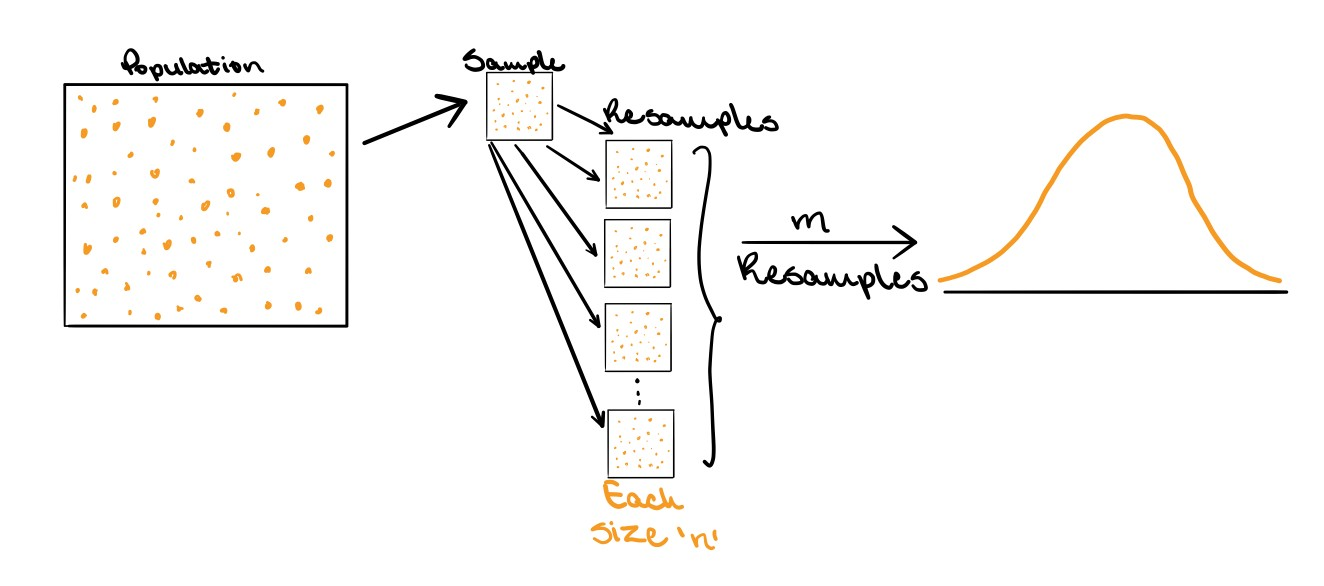
\includegraphics[width=0.7\textwidth]{figures/stats/bootstrapping.jpeg}
\caption{
Illustration of the bootstrapping method
by \href{https://towardsdatascience.com/bootstrapping-statistics-what-it-is-and-why-its-used-e2fa29577307}{Trist'n Joseph}.
Note that the $m$ resamples are done with replacement.
The final bootstrapped distribution is built by measuring the statistic in question on all of the bootstrapped samples,
and can be used to estimate the statistic's uncertainty.
}
\label{fig:bootstrapping}
\end{figure}

%%%%%%%%%%%%%%%%%%%%%%%%%%%%%%%%%%%%%%%%%%%%%%%%%%%%%%%%
\subsection{Hypothesis Testing}
\label{stats:bootstrapping:hypo}

As we can construct confidence intervals, bootstrapping can also be used for hypothesis testing.
N{a\"i}vely we can test the null hypothesis by checking if the value in question,
typically \num{0}, lands within the confidence interval or not.
We can also estimate the \pvalue of a parameter by shifting the original sample distribution such that
it satisfies the null hypothesis, \eg shift all the data points by $\delta$ such that the sample has $\expval{x} = \num{0}$.
We then bootstrap the shifted sample to produce the bootstrapped distribution as normal.
The \pvalue is then the proportion of the bootstrapped distribution
with values differing from the null hypothesis by the observed difference or more,
\eg $P\left(\delta \leq \abs{x}\right)$ in the prior example.

%%%%%%%%%%%%%%%%%%%%%%%%%%%%%%%%%%%%%%%%%%%%%%%%%%%%%%%%
\subsection{Poisson Bootstrapping}
\label{stats:bootstrapping:poisson}

For large sample sizes $n$, instead of drawing $m$ bootstrap samples with replacement,
which can be computationally expensive,
we can use the single sample,
but give each data point a weight $w$ drawn
from the Poisson distribution with $\lambda = 1$.
The set of weights is then generated $m$ times.
Formally, the methods are equivalent as for large $n$
the binomial probability of including a given data point approaches the Poisson probability with $\lambda = 1$.
Poisson Bootstrapping is commonly used in particle physics,
in particular see the direct balance $\gamma\text{+Jet}$ calibration
in the dissertation \cite{mepland_dissertation}, Appendix E.1.4.

%%%%%%%%%%%%%%%%%%%%%%%%%%%%%%%%%%%%%%%%%%%%%%%%%%%%%%%%
%%%%%%%%%%%%%%%%%%%%%%%%%%%%%%%%%%%%%%%%%%%%%%%%%%%%%%%%
\section{Maximum Likelihood Estimation (MLE)}
\label{stats:MLE}

Maximum likelihood estimation (MLE) is a method
of choosing the optimal parameters of a probability distribution
to match some set of observed data.
As the name suggests, MLE works by maximizing the likelihood of observing the given data.
Note that the terms likelihood and probability are closely related, but different, in this context.
Here probability refers to the probability of observing $x$ given parameters $\bm{\beta}$, $P\left(x \mid \bm{\beta}\right)$,
while likelihood refers to the likelihood of the distribution having parameters $\bm{\beta}$ given an observation $x$, $L\left(\bm{\beta} \mid x\right)$.
$L$ and $P$ are both equal to relevant probability distribution,
such as \cref{eq:stats:gaus:P} for the Gaussian distribution,
but which variables are independent and dependent changes.

As we wish to maximize the likelihood with respect to $\bm{\beta}$,
we will be taking partial derivatives and finding where they equal zero, $\partial_{\bm{\beta}} L = 0$.
In practice, likelihood functions are complicated\footnote{The value of $L$
is often close to $0$, making lack of precision an issue when doing computations.
$\log\left(L\right)$ is larger and also helps address this problem.} and
it is easier to maximize the log-likelihood $\log\left(L\right)$,
which has the same maximum as the original likelihood $L$,
but removes exponents and turns multiplication in to addition.
Generally there are $m$ points $\mathbf{x}_{i}$, each with $n$ dimensions, in a given dataset,
thus we are solving \cref{eq:MLE} for $\bm{\beta} = \hat{\bm{\beta}}_{\text{MLE}}$:

\begin{subequations}\label{eq:MLE}
\begin{align}
0 &= \partial_{\bm{\beta}} \, L\left(\bm{\beta} \mid \mathbf{x}\right) \label{eq:MLE:L} \\
\implies 0 &= \partial_{\bm{\beta}} \log\left(L\left(\bm{\beta} \mid \mathbf{X}\right)\right) = \partial_{\bm{\beta}} \, \log\left(\prod_{i=1}^{m} \, P\left(\mathbf{x}_{i} \mid \bm{\beta}\right)\right) \label{eq:MLE:log_L} \\
&= \sum_{i=1}^{m} \, \partial_{\bm{\beta}} \log\left(P\left(\mathbf{x}_{i} \mid \bm{\beta}\right)\right) \label{eq:MLE:log_L_sum}
\end{align}
\end{subequations}

In practice, it is unlikely that a closed form solution for $\hat{\bm{\beta}}_{\text{MLE}}$ can be found
and numerical optimizers, such as gradient descent, are used instead.
Under certain conditions it can be shown that as $n \to \infty$ the MLE converges to $\hat{\bm{\beta}}$,
\ie in the limit $n \to \infty$ no consistent estimator
has a lower MSE\footnote{More formally, the MLE achieves the Cram\'er--Rao lower bound.}.
Lastly, while the MLE is usually a biased estimator, see \cref{additional:stats:bias},
the bias is also reduced as $n \to \infty$.

%%%%%%%%%%%%%%%%%%%%%%%%%%%%%%%%%%%%%%%%%%%%%%%%%%%%%%%%
\subsection{Exponential Distribution Example}
\label{stats:MLE:exp_ex}

We can use MLE to find the optimal $\hat{\lambda}_{\text{MLE}}$ of
the exponential distribution \cref{eq:stats:exp:P}
given a dataset of $m$ points, $x_{i}$, in 1 dimension:

\begin{subequations}\label{eq:MLE:exp_ex}
\begin{align}
0 &= \sum_{i=1}^{m} \partial_{\lambda} \log\left(P\left(x_{i} \mid \lambda\right)\right) = \sum_{i=1}^{m} \partial_{\lambda} \log\left(\lambda e^{-\lambda x_{i}}\right), \label{eq:MLE:exp_ex:log_L_sum} \\
&= \sum_{i=1}^{m}\partial_{\lambda} \left( \log\left(\lambda\right) -\lambda x_{i}\right) = \sum_{i=1}^{m} \frac{1}{\lambda} - x_{i} = \frac{m}{\lambda} - \sum_{i=1}^{m} x_{i}, \label{eq:MLE:exp_ex:solve} \\
\implies \hat{\lambda}_{\text{MLE}} &= \frac{m}{\sum_{i=1}^{m} x_{i}} = \frac{1}{\expval{x}}. \label{eq:MLE:exp_ex:lambda}
\end{align}
\end{subequations}

For another example of MLE see logistic regression \cref{eq:logistic:L_Pr}.

%%%%%%%%%%%%%%%%%%%%%%%%%%%%%%%%%%%%%%%%%%%%%%%%%%%%%%%%
%%%%%%%%%%%%%%%%%%%%%%%%%%%%%%%%%%%%%%%%%%%%%%%%%%%%%%%%
\section{Maximum A Posteriori (MAP)}
\label{stats:MAP}
% TODO In maximum \aposteriori (MAP) estimation
% TODO MLE is a special case of MAP with a uniform prior
